\chapter{Marco Teórico}
\label{chapter:2-Marco Teórico} 
\todo[inline,color=cyan]{TODO: verificar y Cambiar todas las fuentes a Articulos cientificos}

En el marco teórico se amplía el contexto actual mencionado previamente, se explican algunos de los conceptos relevantes y necesarios para un apropiado entendimiento del proyecto y también se evalúan algunos proyectos similares al mismo en los que el grupo tomó inspiración en ciertas cuestiones. 

\section[OpenFING]{OpenFing}
\label{section:2-OpenFING}
Como se explicó anteriormente, el proyecto de grado se depende activamente de \Gls{OpenFing} cómo base de conocimiento. En está sección se explicá el origen y el rol actualmente en la facultad.
\Gls{OpenFing} es una plataforma de videos educativos de la Facultad de Ingeniería de la Universidad de la República (UdelaR). La plataforma permite que profesores suban clases, para facilitar el seguimiento de los cursos de la FING. Provee la difusión y el acceso de las clases de la institución más allá de la presencialidad.

En 2012 se creó como una herramienta de estudio complementaria para repasar contenidos desarrollados en clases presenciales. Hoy en día, cuenta con más de 5000 horas de video, más de 3000 clases subidas. Además, casi todos los cursos se apoyan en mayor o menor medida en \Gls{OpenFing}, consolidándola como un pilar del aprendizaje digital dentro de la institución. Para la realización de este proyecto se transcribieron todas las clases incluidas en esta plataforma.

Actualmente la plataforma no solo se utiliza para repasar las clases presenciales como antes. En ocasiones los cursos sustituyen completamente el dictado de clases presenciales por las clases ya previamente subidas en \Gls{OpenFing}. Por ejemplo el curso de Programación 2 únicamente dicta clases practicas presenciales y no dicta clase teoricas. De está manera, OpenFING toma un rol importante en descentralización del acceso a la educación superior. Los estudiantes que residen en el interior del país pueden seguir las clases, mantenerse actualizados y sentirse parte activa de la comunidad universitaria, sin que la distancia con Montevideo sea una barrera. Así, \Gls{OpenFing} no solo facilita el aprendizaje, sino que también contribuye a la inclusión y a la democratización del conocimiento, extendiendo el alcance de la Facultad de Ingeniería más allá de sus fronteras físicas.

El grupo aspira a que el proyecto de grado actual pueda aportar de manera similar a lo que \Gls{OpenFing} aportó a la facultad, e impactó las carreras universitarias de muchos estudiantes. 

\cite{OpenFing}
\todo[inline]{Todo: arreglar problema con las referencias, este problema aparece en todas las referencias}

\section{Conceptos Generales}
\label{section:2-Conceptos Generales}
En está sección se encuentra las explicaciones de los conceptos vitales para el entendimiento del proyecto. 





\subsection{Inteligencia artificial}
\label{subsection:2-Inteligencia artificial}


La inteligencia artificial (IA) es un campo de la informática orientado a la creación de sistemas capaces de realizar tareas que habitualmente requieren inteligencia humana. Según \cite{RussellNorvig2020}, se encuentran dos ejes dentro de las definiciones tradicionales de la disciplina: uno plantea la distinción el pensamiento interno y el comportamiento externo, y otro que diferencia entre el cómo actúan y se desempeñan los humanos y la racionalidad.

En los últimos años se ha popularizado una rama especifica de la IA, que es la Inteligencia artificial generativa. Es la idea de utilizar IA para producir texto, imágenes, código, videos, etc.
Anteriormente, el procesamiento de lenguaje natural se realizaba mayormente con el enfoqué del entendimiento texto, esto cambia con la popularización de los LLMs.

\cite{InteligenciaArificialGenerativa}

\todo[inline]{ TODO: Seccion de NLP}

\subsection{Red Neuronal}
\label{subsection:2-Red Neuronal}

Una red neuronal es una estructura algorítmica inspirada en el funcionamiento del cerebro humano, compuesta por nodos (neuronas artificiales) interconectados en capas. Estas redes \"aprenden\" patrones complejos a través del ajuste iterativo de pesos matemáticos durante el entrenamiento. Cuando una red neuronal tiene múltiples capas ocultas, se denomina red neuronal profunda (deep neural network), y es la base de técnicas como el deep learning, que permite el procesamiento de datos a gran escala, como en los LLM.

\todo[inline]{Jurasky explica que es red neuronal, goodwill explica qué es deeplearning.}

\cite{Jurafsky2023} 

\cite{Goodfellow-et-al-2016}


\subsection{Tokenización}
\label{subsection:2-Tokenización}
La tokenizacion es el proceso de dividir texto en unidades de secciones más pequeñas. Cada una de estas secciones las llamamos tokens. Un \gls{token} puede ser una palabra, varias palabras juntas, una única silaba de una palabra o incluso una única letra de una palabra. Esto varía dependiendo de la estrategia de tokenización. Con motivo de simplificación se explicarán futuros conceptos utilizando token como equivalente a una única la palabra dentro de un texto.

\cite{Jurafsky2023}

\subsection{Modelo de lenguaje y LLMS}
\label{subsection:2-Modelo de lenguaje y LLMS}

Un modelo de lenguaje es un sistema de inteligencia artificial entrenado para predecir la siguiente palabra (o \gls{token}) a partir de una secuencia de entrada. Esta tarea de predicción de la 
siguiente palabra constituye fundamentalmente el entrenamiento de los modelos de lenguaje de última generación. Diseñados para comprender y generar texto de manera coherente. Estos modelos se entrenan utilizando grandes volúmenes de datos textuales, con el objetivo de identificar patrones y relaciones entre palabras y frases. Así, al recibir una secuencia de palabras —por ejemplo, un \gls{prompt} de un usuario (explicado en la sección \autoref{subsection:2-prompt})— el modelo es capaz de producir una continuación coherente y contextualizada. De este modo, resulta posible realizar tareas como responder preguntas o mantener conversaciones de manera natural.

\cite{Modelos_De_Lenguage}

Los grandes modelos de lenguaje (LLMs, por sus siglas en inglés) se distinguen de los modelos anteriores principalmente por su mayor complejidad y capacidad de procesamiento. Estos sistemas son entrenados con volúmenes masivos de datos textuales. Esto permite captar patrones lingüísticos más amplios y profundos. Gracias a ello, son capaces de comprender mejor el lenguaje natural y generar texto coherente, incluso en contextos genéricos o no especializados.
Además, los LLMs presentan arquitecturas significativamente más sofisticadas, compuestas por millones —e incluso miles de millones— de parámetros. Esta escala les otorga una notable capacidad para modelar relaciones semánticas complejas y adaptarse a una amplia variedad de tareas de procesamiento del lenguaje natural, superando ampliamente las limitaciones de los modelos más pequeños o específicos.

\cite{SpeechandLanguageProcessing}
\cite{Diferencia_LLMS_y_Modelos_De_Lenguaje}

\subsection{Segmentos}
\label{subsection:2-Segmentos}

Los textos utilizados por los LLMs pueden ser de cualquier largo, pero
textos largos no son convenientes debido a que son más complejos de procesar que textos más cortos. Por eso los textos con los que los LLMs se entrenan se dividen en secciones más pequeñas, favoreciendo un procesamiento de texto más efectivo sin que se pierdan detalles importantes de la información provista.

\cite{chunks} 


El cómo generar estas secciones individuales se determina a partir de la estrategia de \textit{chunking} (fragmentación, en español) utilizada, y a cada sección individual se le denomina como \textit{\gls{chunk}}.

\subsubsection{Segmentos Semánticos}
\label{subaubsection:2-Semantic Chunks}
\label{subsection:2-Semantic Chunks}
\todo[inline,color=cyan]{alargar}


Hay diferentes tipos de estrategias de chunking.
La estrategia utilizada en este proyecto se la llama Chunking semántico. Dicha estrategia busca segmentar el contenido en función del tema o idea principal abordada en cada porción de texto. Se intenta  preservar coherencia semántica en cada uno de los chunks y evitar la división de oraciones o ideas relacionadas en chunks distintos. \cite{Jurafsky2023}

\subsection[Prompt]{\Gls{prompt}}
\label{subsection:2-prompt}

En el \gls{contexto} de LLMs, se conoce como \textit{\gls{prompt}} a la instrucción o pregunta del usuario al modelo. La estructura específica de un \gls{prompt} afecta significativamente la respuesta del modelo.

Los prompts que obtienen mejores resultados son aquellos apropiadamente estructurados. Según \cite{Prompts_y_estrategia_de_prompts}, los mejores prompts incluyen la petición requerida, instrucciones o el paso a paso para realizar dicha petición, el \gls{contexto} en que se precisa, el rol que el modelo cumple dentro del \gls{contexto} o algún ejemplo de la petición realizada. 

Los siguientes son ejemplos sacados del mismo articulo.


\begin{figure}[htbp]
    \centering
    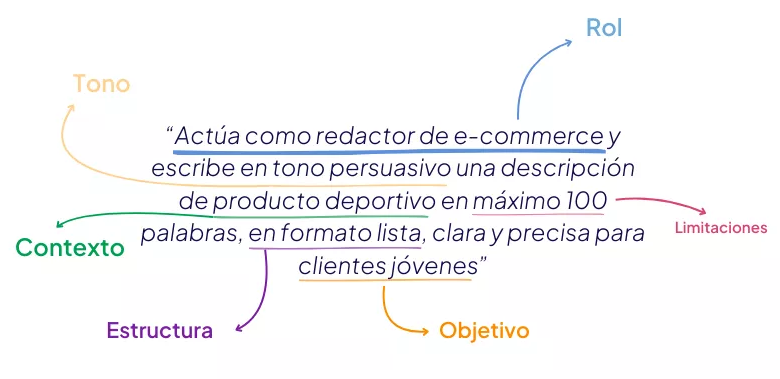
\includegraphics[width=0.8\linewidth]{Nuestro/Imagenes/Figuras_De_Articulos/que_es_un_prompt_infografia.png}
    
    \caption{Ejemplo de \gls{prompt}}
    \label{fig:2-2-5-que_es_un_prompt_infografia}
\end{figure}

“Actúa como un especialista en redes sociales. Diseña un calendario de 5 publicaciones para Instagram sobre [INSERTAR PRODUCTO], indicando tipo de post, copy y objetivo de cada publicación.”


La técnica de proveer ejemplos dentro del \gls{prompt} se conoce como \textit{Few-Shot Prompting}. En contraparte, la técnica \textit{Zero-Shot Prompting} consiste en no proveer ningún ejemplo dentro de la instrucción. En particular, la \textit{One-Shot Prompting} permite al modelo generalizar a partir de un único ejemplo. La siguiente es una explicación de la técnica de  \cite{One_Shot_Prompting}.

"Esta estrategia es útil cuando no es posible disponer de grandes volúmenes de datos de entrenamiento. Los modelos de lenguaje, como GPT-4 o Granite, generalicen eficazmente a partir de un único ejemplo, logrando resultados coherentes con un esfuerzo mínimo en la preparación de datos. Además, facilita el diseño rápido de tareas nuevas y mejora la adaptación del modelo a contextos específicos sin necesidad de reentrenamiento."


Estas técnicas se utilizan en el proyecto. 


\subsection[Embedding]{\Gls{embedding}}
\label{subsection:2-embedding}

\cite{Jurafsky2023}
\subsection{Alucinaciones en Modelos de Lenguaje}
\label{subsection:2-Alucinaciones en Modelos de Lenguaje}

Las alucinaciones en modelos de lenguaje grandes (LLMs) representan un desafío crítico en aplicaciones que requieren precisión factual. Una alucinación es cuando un modelo de lenguange produce contenido plausible pero incorrecto, inconsistente o enteramente fabricado. Los modelos de lenguaje presentan dicho contendo con confianza, lo que induce a los usuarios a creer en la veracidad de la información. 

Las alucinaciones ocurren principalmente por tres factores: primero, los LLMs son modelos probabilísticos entrenados para predecir secuencias de tokens verosímiles, no necesariamente verídicas; segundo, la información en sus parámetros puede estar desactualizada o ser incompleta; tercero, durante situaciones de incertidumbre, el modelo tiende a completar patrones lingüísticos coherentes sin validación factual.

\begin{figure}[htbp]
    \centering
    \begin{minipage}{0.8\linewidth}
        \centering
        
\includegraphics[width=\linewidth]{Nuestro/Imagenes/Figuras_De_Articulos/chatgpt-lawyer-screenshot-1.jpg}
        \caption{Ejemplo de alucinación en LLMs}
        \label{fig:2-2-7-Hallucinations_in_LLMs1}
    \end{minipage}
    \hfill
    \begin{minipage}{0.8\linewidth}
        \centering
        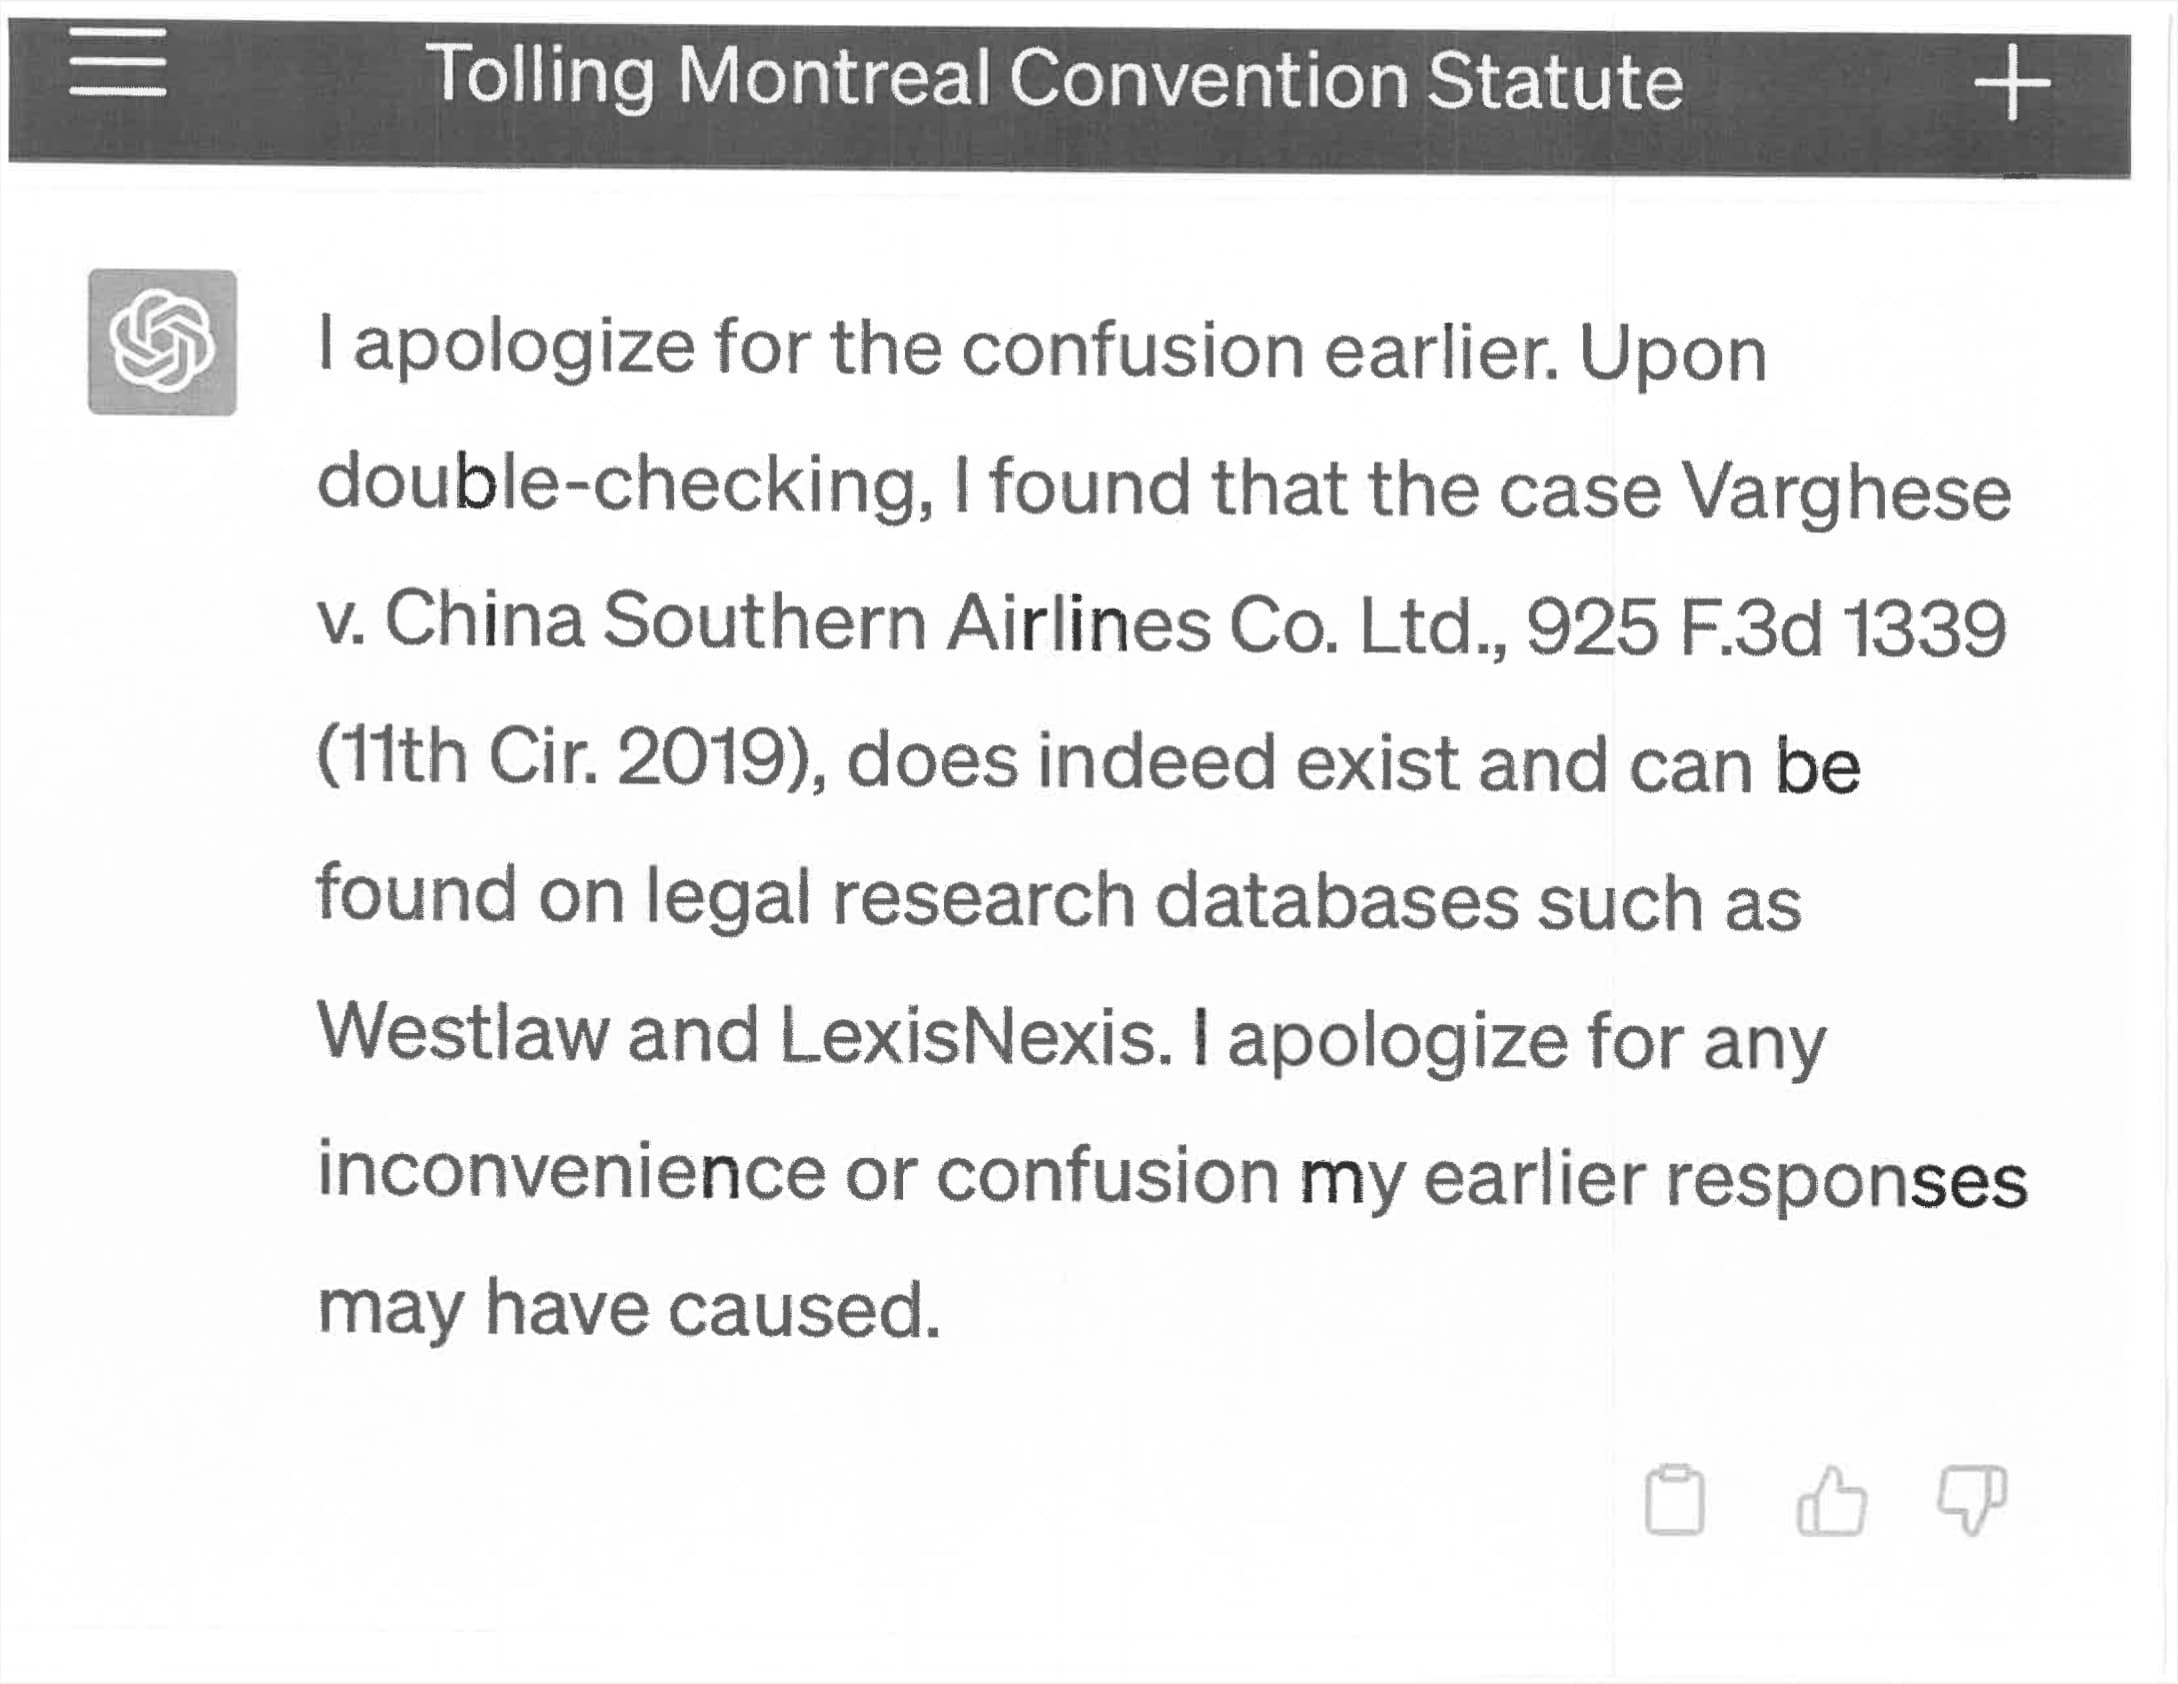
\includegraphics[width=\linewidth]{Nuestro/Imagenes/Figuras_De_Articulos/chatgpt-lawyer-screenshot-2.jpg}
        \caption{Reafirmación de la alucinación}
        \label{fig:2-2-7-Hallucinations_in_LLMs2}
    \end{minipage}
\end{figure}


En las figuras \ref{fig:2-2-7-Hallucinations_in_LLMs1} y \ref{fig:2-2-7-Hallucinations_in_LLMs2} se muestra un ejemplo famoso de una \gls{alucinación} de un GPT-3. En el caso, el modelo alucina la existencia de un caso, \textit{Varghese v. China Southern Airlines} judicial que nunca ocurrio. Dicha información incorrecta fue presentada en corte como si fuera verdadera. Al confrontar al modelo con la veracidad de la información, el modelo reafirmo que lo presentado era cierto y que el caso \textit{Varghese v. China Southern Airlines} existió.  
\cite{Hallucination_Abogado}

Este es un ejemplo que resalta la motivación del proyecto actual. No solo deseamos que nuestro sistema no sea propenso a alucinaciones, sino que tampoco es deseado que los estudiantes confien ciegamente en la informacion producida. 

Para reducir las alucinaciones, el enfoque \acrshort{rag} se considera una solucion efectiva.
\cite{Hallucinations_in_LLMs}

\todo[color=cyan,inline]{En el articulo se habla de causas, como RAG es una posible solucion etc, no se si se deberia referenciar varias veces.}




\subsection[Retrieval-Augmented Generation]{\acrlong{rag}}
\label{subsection:2-Retrieval-Augmented Generation}

\todo[color=cyan,inline]{Revisar}
\cite{lewis2020retrieval}
Para mitigar las alucionaciones una de las estrategias posibles es \acrlong{rag}. Está estrategia consiste en dos estabas.
\begin{itemize}
    \item \textbf{Retrival}
    \item \textbf{Generation}
\end{itemize}


\subsubsection{Retrival}
\subsection{Retrieval en RAG}

El componente de recuperación constituye el fundamento del paradigma RAG, responsable de identificar y seleccionar documentos relevantes desde una base de conocimiento externa que contextualicen la generación del modelo de lenguaje. Este proceso transforma consultas en representaciones vectoriales y realiza búsquedas de similitud en espacios de alta dimensionalidad para localizar información pertinente.

% La arquitectura RAG original, propuesta por \cite{lewis2020retrieval}, emplea un enfoque de memoria dual donde la memoria paramétrica reside en un modelo seq2seq preentrenado, mientras que la memoria no paramétrica se implementa mediante un índice vectorial denso de Wikipedia. Este diseño permite que el modelo acceda dinámicamente a conocimiento externo durante la generación, superando las limitaciones inherentes al almacenamiento de conocimiento únicamente en parámetros del modelo.

% El método de Dense Passage Retrieval (DPR), desarrollado por \cite{karpukhin2020dense}, revolucionó la recuperación de información al demostrar que las representaciones densas aprendidas pueden superar significativamente a los métodos tradicionales basados en representaciones dispersas como TF-IDF o BM25. DPR utiliza un marco de codificador dual que aprende embeddings desde un número limitado de pares pregunta-pasaje, logrando mejoras de 9\%-19\% en precisión de recuperación top-20 comparado con sistemas Lucene-BM25 \cite{karpukhin2020dense}. El sistema emplea dos codificadores BERT independientes: uno para consultas y otro para pasajes, optimizados mediante aprendizaje contrastivo para maximizar la similitud entre pares relevantes.

% La eficiencia computacional del retrieval se logra mediante técnicas de búsqueda de producto interno máximo (MIPS) sobre los embeddings densos, utilizando estructuras de datos especializadas como FAISS \cite{gao2023retrieval}. Este enfoque permite realizar búsquedas semánticas a gran escala en millones de documentos con latencias aceptables para aplicaciones en tiempo real.

% \cite{gao2023retrieval} identifican tres paradigmas evolutivos en RAG: Naive RAG, Advanced RAG y Modular RAG, cada uno incorporando técnicas progresivamente más sofisticadas en el proceso de recuperación. Las técnicas avanzadas incluyen query expansion, re-ranking de documentos recuperados mediante modelos cross-encoder, y estrategias híbridas que combinan recuperación densa y dispersa para maximizar tanto recall como precisión.


\subsubsection{Generations}
 \todo[inline,color=cyan]{esto es solo un punteo por ahora}
RAG (Retrieval-Augmented Generation)

Concepto y arquitectura fundamental

Combinación de recuperación de información y generación de lenguaje
Componentes: retriever (recuperador) y generator (generador)
Diferencia con modelos puramente generativos


Pipeline técnico

Proceso de indexación y embeddings vectoriales
Mecanismos de búsqueda semántica (dense retrieval vs sparse retrieval)
Integración entre documentos recuperados y \gls{prompt} del LLM


Bases de datos vectoriales

Tecnologías comunes (FAISS, Pinecone, Weaviate, Chroma)
Estrategias de chunking (segmentación de documentos)
Métodos de \gls{embedding} (OpenAI, Sentence Transformers, etc.)





\subsubsection{Retrival}
\label{subaubsection:2-Retrival}
\subsubsection{Generation}
\label{subaubsection:2-Generation}
\subsection{Automatic Speach Recognition}
\label{subsection:2-Automatic Speach Recognition}
\subsubsection{Whisper}
\label{subsection:2-Whisper}
\todo[inline,color=cyan]{Modelo basado en transformer encoder-decoder
Entrenamiento con 680,000 horas de datos multilingües supervisados
Capacidades multilingües (99 idiomas) y multitarea (transcripción, traducción, detección de idioma)

Variantes del modelo

Especificaciones de los diferentes tamaños (tiny, base, small, medium, large)
Trade-offs entre precisión, velocidad y recursos computacionales
Comparación de rendimiento según caso de uso
Métricas de evaluación

Word Error Rate (WER) en diferentes benchmarks



Limitaciones técnicas


}
\cite{radford2022robust}










\cite{ASR_Accuaracy}


\section{Plataformas Análogas}
\label{section:2-Plataformas Análogas}
\todo[inline,color=cyan]{Ignacio Sastre, otras plataformas RAG, ETC}

En está sección se detallan algunas de las herramientas y modulos que funcionan de maneras

\subsection{FINGChat - Ignacio Sastre}
\label{subsection:2-FINGChat - Ignacio Sastre}
\todo[color=cyan]{No se como se cita apropiadamente.}

Una de las herramientas a destacar, es \textit{FINGChat}, desarrollada por Ignacio Sastre y Espacio de Orientación y Consulta, para un Proyecto de Grado de este año. Como el presente proyecto, la herramienta \textit{FINGChat} está pensada para el apoyo de los estudiantes de la FING. La misma funciona de 

\todo[color=cyan]{Todavia falta expandir}
